\begin{figure}[t]
\centering
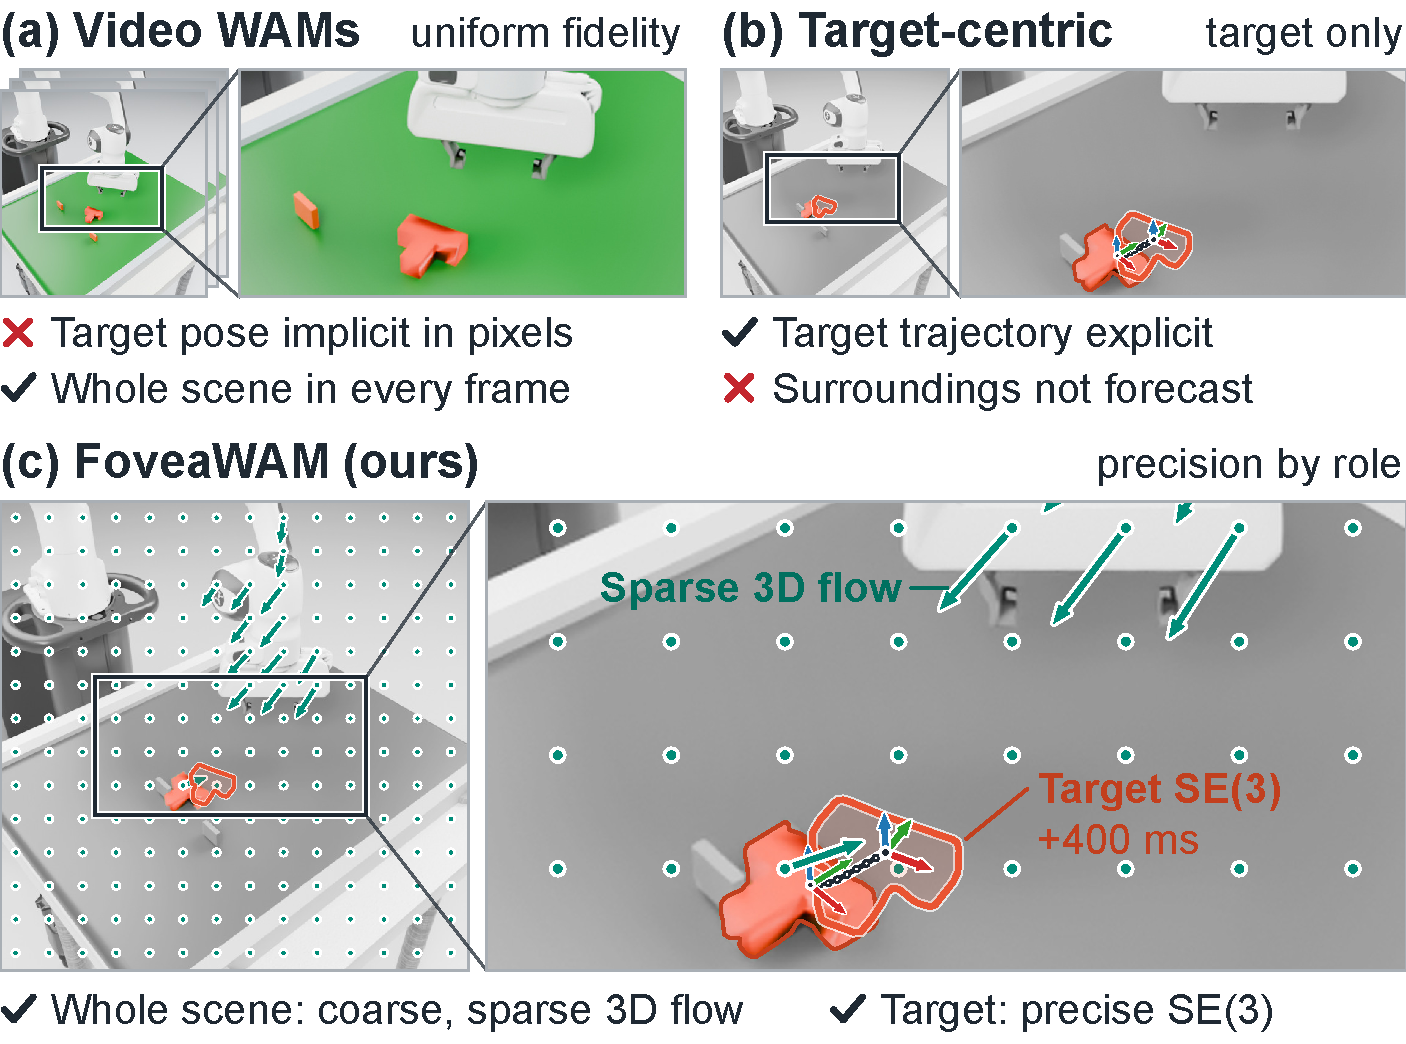
\includegraphics[width=\columnwidth]{figures/paradigms/paradigms.pdf}
\caption{\textbf{预测精度分配在哪里。}
用同一个 \bench 录制场景示意三种预测表示（agent 视角，方框内区域放大显示）。
(a) 视频 WAM 以统一的精细程度预测未来帧或隐变量，目标的度量位姿仍隐含其中 \cite{dreamzero,openwam_alpha}。
(b) 以目标为中心的预测器仅预测目标轨迹 \cite{domino,spot}。
(c) \ours 读取一帧 RGB-D 与目标的 SE(3) 历史，以 \cfgContextGrid{} 网格上的稀疏 3D 流粗略预测整个场景（青色，圆点表示位移 $\leq 2$\,mm），其中只有一个采样点落在目标上。模型同时精确预测目标的 SE(3) 轨迹（橙色，坐标轴为当前与 $+400$\,ms 的位姿）。两种预测均用于训练监督，在推理时跳过。叠加内容来自录制数据。}
\label{fig:paradigms}
\end{figure}
